
\section{State-Space Representations}

\begin{frame}
\frametitle{State Space Modeling: Example}

Assume we have the following spring system: \\
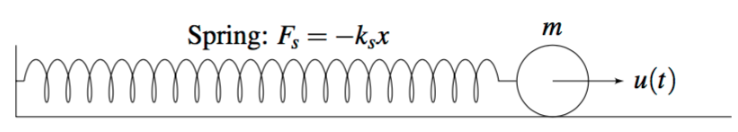
\includegraphics[scale=0.5]{./images/spring.png} \\ \pause
We can model the system as a linear continuous time state space model: \\
$\frac{d}{dt}\vec{x}(t) = A\vec{x}(t) + \vec{b}u(t)$ \\
$\vec{y}(t) = C\vec{x}(t)$ \\
in which: \\
$\vec{x}(t) = 
\begin{bmatrix}
x(t) \\
v(t)
\end{bmatrix}$, 
$A = 
\begin{bmatrix}
0 & 1 \\
-\frac{k_{s}}{m} & 0
\end{bmatrix}$, 
$\vec{b} = 
\begin{bmatrix}
0 \\
1
\end{bmatrix}$, and
$C = 
\begin{bmatrix}
0 & 1
\end{bmatrix}$
\end{frame}

\begin{frame}
\frametitle{State Space Modeling:}
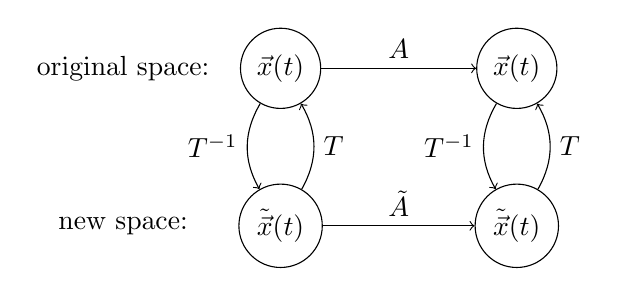
\begin{tikzpicture}
    \node at (-2, 2) {original space:};
    \node at (-2, 0) {new space:};

    \node[draw,circle] (x) at (0, 2) {\(\vec x(t)\)};
    \node[draw,circle] (dx) at (3, 2) {\(\ddt{}\vec x(t)\)};
    \node[draw,circle] (xt) at (0, 0) {\(\tilde{\vec{x}}(t)\)};
    \node[draw,circle] (dxt) at (3, 0) {\(\ddt{}\tilde{\vec{x}}(t)\)};

    \path[->] (x) edge node [above] {\(A\)} (dx);
    \path[->] (xt) edge node [above] {\(\tilde A\)} (dxt);
    \path[->] (x) edge [bend right] node [left] {\(T^{-1}\)} (xt);
    \path[->] (xt) edge [bend right] node [right] {\(T\)} (x);
    \path[->] (dx) edge [bend right] node [left] {\(T^{-1}\)} (dxt);
    \path[->] (dxt) edge [bend right] node [right] {\(T\)} (dx);
\end{tikzpicture}

Always apply operations to right side first
\[\tilde{A} = T^{-1}AT \]
\[\tilde{\vec{x}}(t) = T^{-1}\vec{x}(t)\]
\end{frame}

\begin{frame}
\frametitle{State Space Modeling Procedure:}
\begin{enumerate}
    \item Set up differential equation of the form: $\ddt{}\vec{x}(t) = A\vec{x}(t) + \vec{b}u(t)$  \pause
\item Find $\lambda_i$ of \(A\); let $\tilde{A} = \begin{bmatrix}
\lambda_{1} & 0 & \cdots & 0 \\
0 & \lambda_{2} & 0  & \vdots \\
\vdots & 0 & \ddots & 0 \\
0 & \cdots & 0 & \lambda_{n} \\
\end{bmatrix}$ \pause
\item Find eigenvectors $\vec{v}_i$ of \(A\); let
$T = \begin{bmatrix}
\vec{v_{1}} & \vec{v_{2}} & \cdots & \vec{v_{n}}
\end{bmatrix}$ \pause
\item Convert $\vec{x}(t)$ to $\tilde{\vec{x}}(t)$ using:
$\tilde{\vec{x}}(t) = T^{-1}\vec{x}(t)$ \pause
\item Solve $\frac{d}{dt}\tilde{\vec{x}}(t) = \tilde{A}\tilde{\vec{x}}(t) + T \vec{b} u(t)$ \pause
\item Convert solution back to $\vec{x}(t)$ 
\end{enumerate}
\end{frame}

\begin{frame}
\frametitle{State Space Modeling:}

Continuous time solution: 
\[
    \tilde{x}(t) = e^{\lambda t} \tilde x(0) + \frac{e^{\lambda t} - 1}{\lambda } u(t) + w(t)
\]

Discrete time solution:
\[
     x_{d}(i+1) = e^{\lambda \Delta} x_{d}(i) + \frac{e^{\lambda \Delta} - 1}{\lambda } u(i) + w(i)
\]
\end{frame}

\begin{frame}
\frametitle{State Space Modeling Example:}

Given the following circuit: 

\begin{tikzpicture}[scale=2]
    \draw (2, 0.75) to [R, *-, l_={\(R_2\)}] (1, 0.75) to [R, *-, l_={\(R_1\)}] (0, 0.75) to [voltage source, v_>={\(V_{in}\)}] (0, 0);
    \draw (1, 0.75) node[label={\(V_1\)}] {} to [C, l={\(C_1\)}] (1, 0) node[ground] {};
    \draw (2, 0.75) node[label={\(V_2\)}] {} to [C, l={\(C_2\)}] (2, 0) node[ground] {};
    %\draw (0, 0) to (1.5, 0) to [C, l=2<\micro\farad>] (1.5, 1) to (0, 1) to [L, l=2<\henry>] (0, 0);
    %\draw (0, 0) to (0.75, 0) to (0.75, 0.0) node[ground] {} to (0.75, 0) to  (1.5, 0) to [C, l=2<\micro\farad>, v_<=\(v\)] (1.5, 1) to (0, 1) to[I=\(i\)] [L, l=2<\henry>] (0, 0);
            \node [ground] (0, 0) {};
\end{tikzpicture}

in which $R_{1} = \SI{2}{\ohm}, R_{2} = \frac{8}{3} \si{\ohm}, C_{1} = \SI{1}{\coulomb}, C_{2} = \frac{3}{2} \si{\coulomb} $ \\
solve equations for $V_{1}$ and $V_{2}$
\end{frame}

